\documentclass[tikz, border=2pt]{standalone}

\usepackage{amsmath,amssymb}
\usepackage{pgfplots}
\pgfplotsset{compat=1.18}
\usepackage{xcolor}

\definecolor{utnblue}{RGB}{0, 51, 102}

\begin{document}
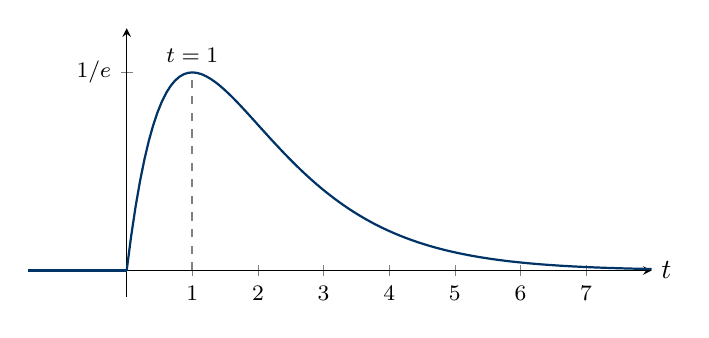
\begin{tikzpicture}
\begin{axis}[
    width=9.5cm, height=5.0cm,
    axis lines=middle,
    enlargelimits=false,
    tick label style={font=\footnotesize},
    label style={font=\small},
    xlabel={$t$},
    every axis x label/.style={at={(ticklabel* cs:1)}, anchor=west},
    xmin=-1.5, xmax=8, ymin=-0.05, ymax=0.45,
    xtick={1,2,3,4,5,6,7},
    ytick={0.3679}, yticklabels={$1/e$},
]
\addplot[utnblue, thick, samples=120, domain=0:8] {x*exp(-x)};
\addplot[utnblue, thick, domain=-1.5:0] {0};
\addplot[gray, dashed, thick] coordinates {(1,0) (1,0.3679)};
\node[font=\footnotesize, anchor=south] at (axis cs:1,0.3679) {$t=1$};
\end{axis}
\end{tikzpicture}
\end{document}
